\chapter{Related Work}
\label{chap:related-work}

Compared to the execution problem, the literature for the order placement problem is sparse (as confirmed by Guo et al. \cite{guo2013optimal}).
In this Chapter, we will provide an overview of the work relied upon for the foundations of this project and for the insights they provided.
We will first consider an empirical study of the general behavior of order placements, which serves as the conceptual basis for this project.
Then, we will present a statistical approach which provides contrast to the subsequent overview of previous machine learning approaches.
todo

\section{Execution/Placement behaviour}
\label{sec:related-execution-behaviour}

Kearns et al. \cite{nevmyvaka2005electronic} determined which limit order price results in the most advantageous execution price.
First, the \textit{expected execution price} is investigated with respect to the placement of the limit order. 
Based on this analysis, the standard deviation of the resulting prices will identify the \textit{risk} that comes with limit order placement. 
Finally, by combining the previous two results, an \textit{efficient pricing frontier} can be drawn which highlights the trade-off between risk and returns.

Regarding the definition stated in Section \ref{sec:execution-placement}, their research can be categorized between order execution and placement.
No splitting of orders was performed, however a time horizon of several hours was chosen, resulting in an evaluation of order placement with an extended time horizon.

\begin{figure}[H]
    \centering
    \makebox[\linewidth]{
        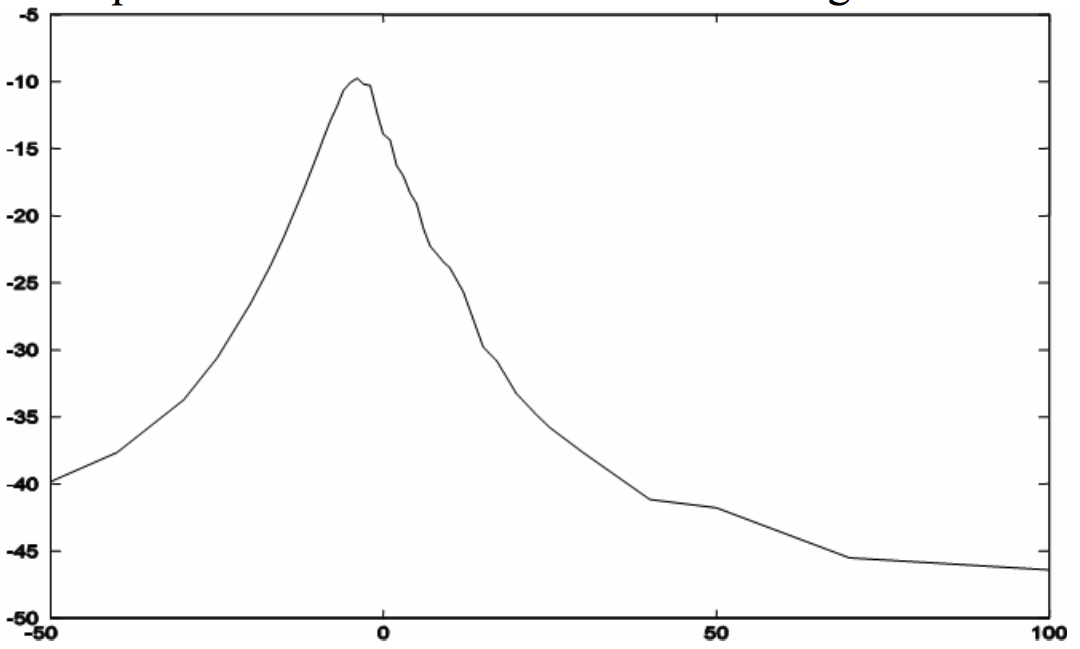
\includegraphics[width=8cm]{kearns-return.png}
    }
    \caption{Taken from \cite{nevmyvaka2005electronic}. An illustration of the pricing strategy that produces the most favorable expected execution price.}
    \label{fig:kearns-return}
\end{figure}

Figure \ref{fig:kearns-return} shows on the y-axis the return as the weighted average price paid of the expected execution price while acquiring 10,000 shares of MSFT within one hour.
The x-axis represents the limit level ranging from -\$50 to +\$100.
As is evident from the figure, the expected execution price is at its most favorable when setting the limit price close to the price of the spread, although only on the buyer side with a price of approximately \$10 lower than what is currently offered.
The return becomes worse when placing orders deeper in the order book (in other words, offering a lower price) as the orders then do not get filled within an hour and instead, the inventory has to be bought by means of a market order at the end of the period.
Likewise, the return can be expected to be lower when placing the order higher in the order book (i.e. deeper in the opposing side of the book, meaning one is willing to pay more).
This is due to the fact that the order is filled instantly by paying a premium.

\begin{figure}[H]
    \centering
    \makebox[\linewidth]{
        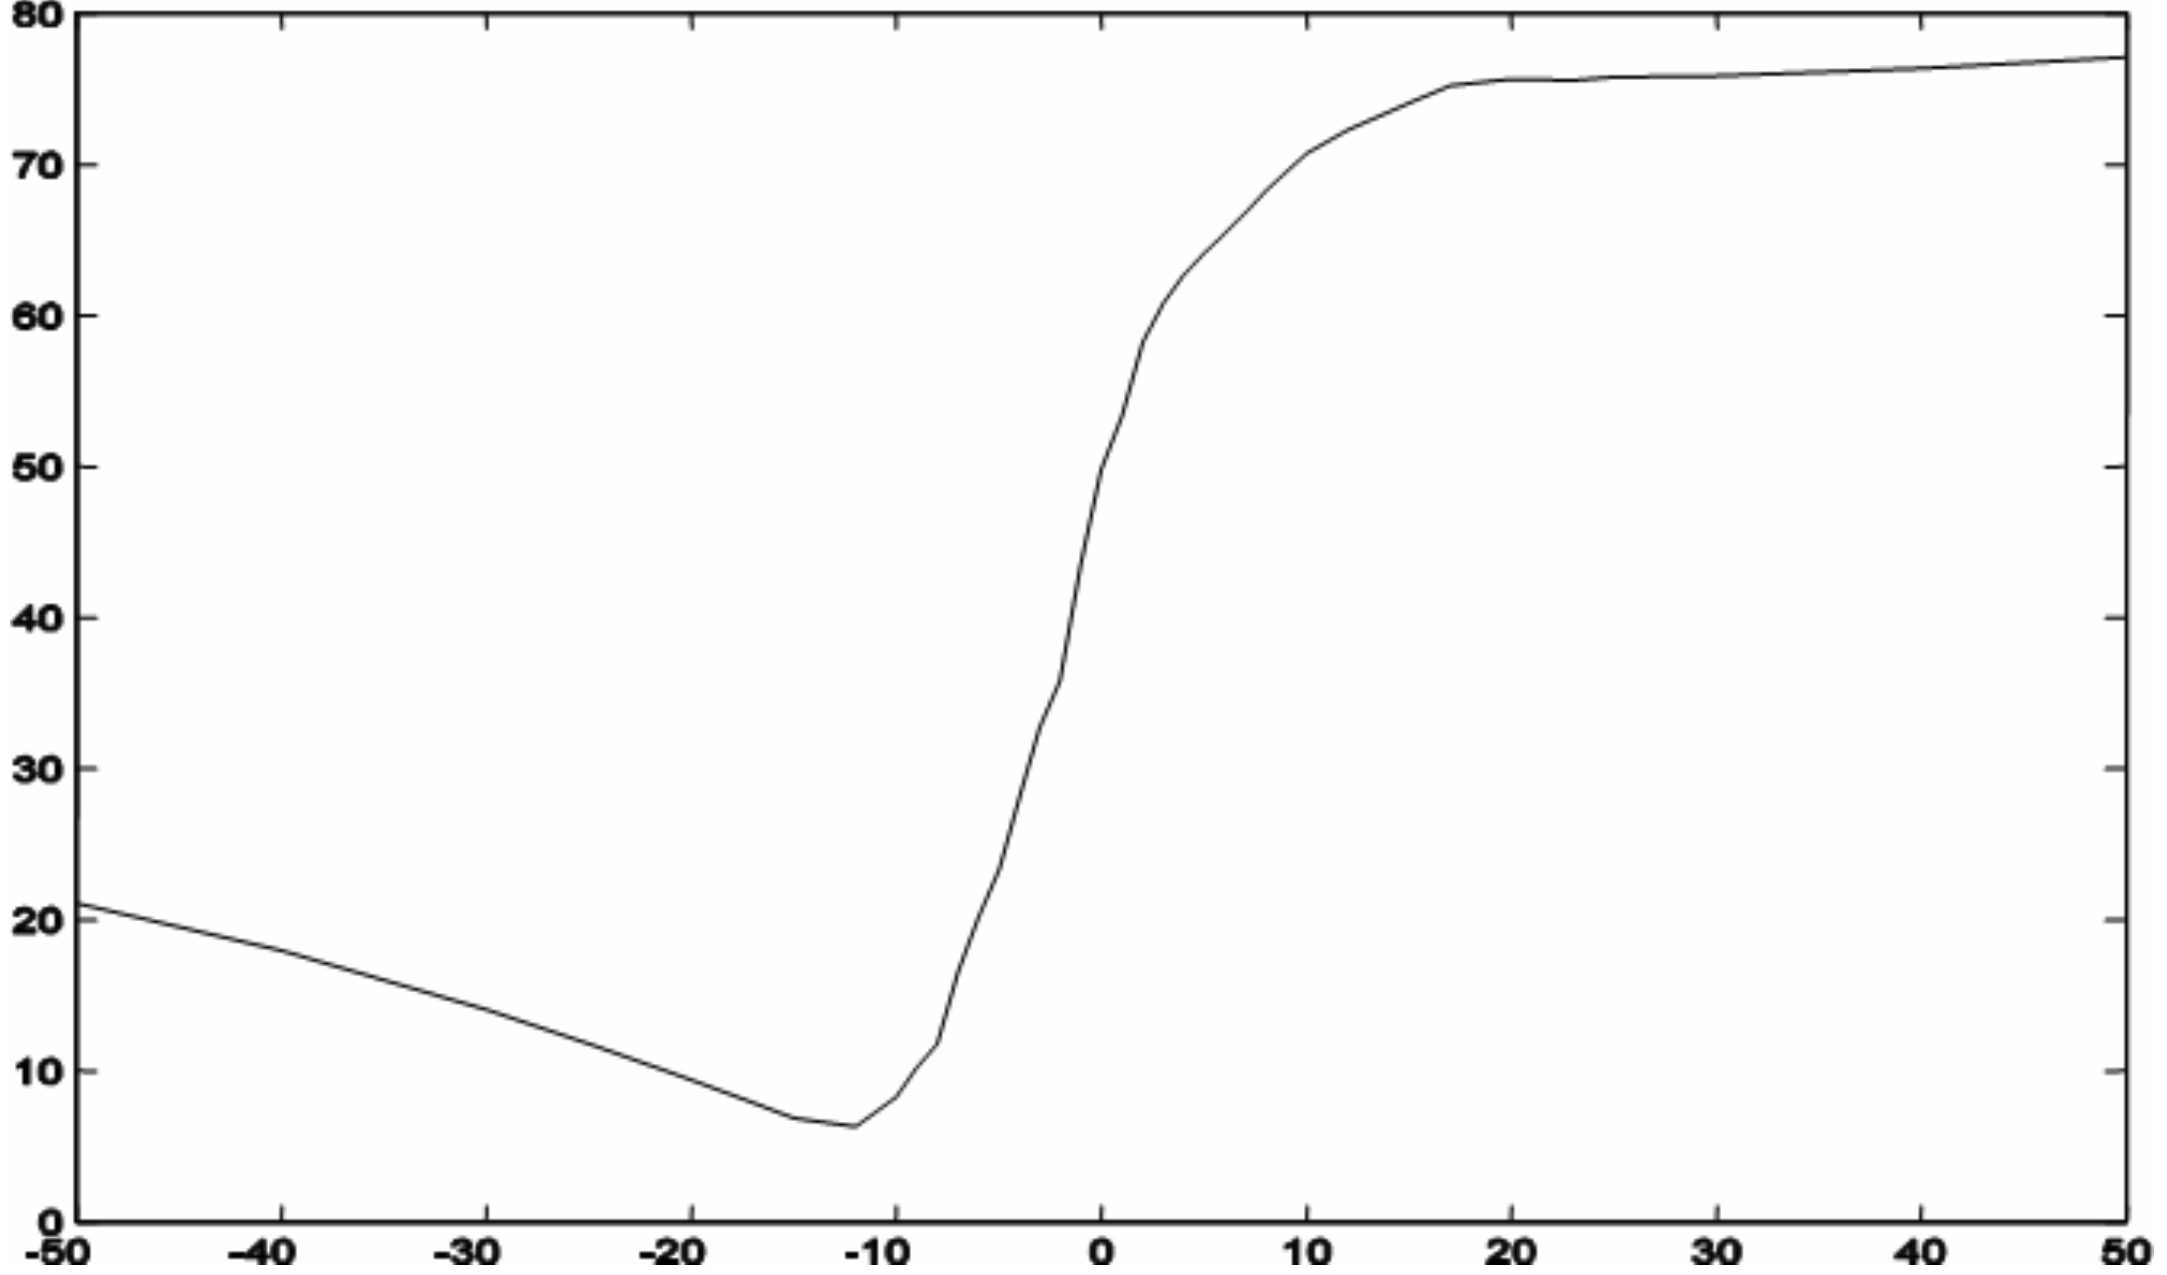
\includegraphics[width=8cm]{kearns-std.png}
    }
    \caption{Taken from \cite{nevmyvaka2005electronic}. An illustration of the uncertainty of the expected execution price.}
    \label{fig:kearns-std}
\end{figure}

Risk is defined as the standard deviation of the returns and is illustrated on the y-axis in Figure \ref{fig:kearns-std}.
This is an important aspect to be considered throughout our project as it illustrates the danger that arises from placing limit orders at less favourable limit levels.
As has been already demonstrated, orders which are placed deep in either side of the book are less likely to be executed and their final prices are therefore necessarily less certain.

\begin{figure}[H]
    \centering
    \makebox[\linewidth]{
        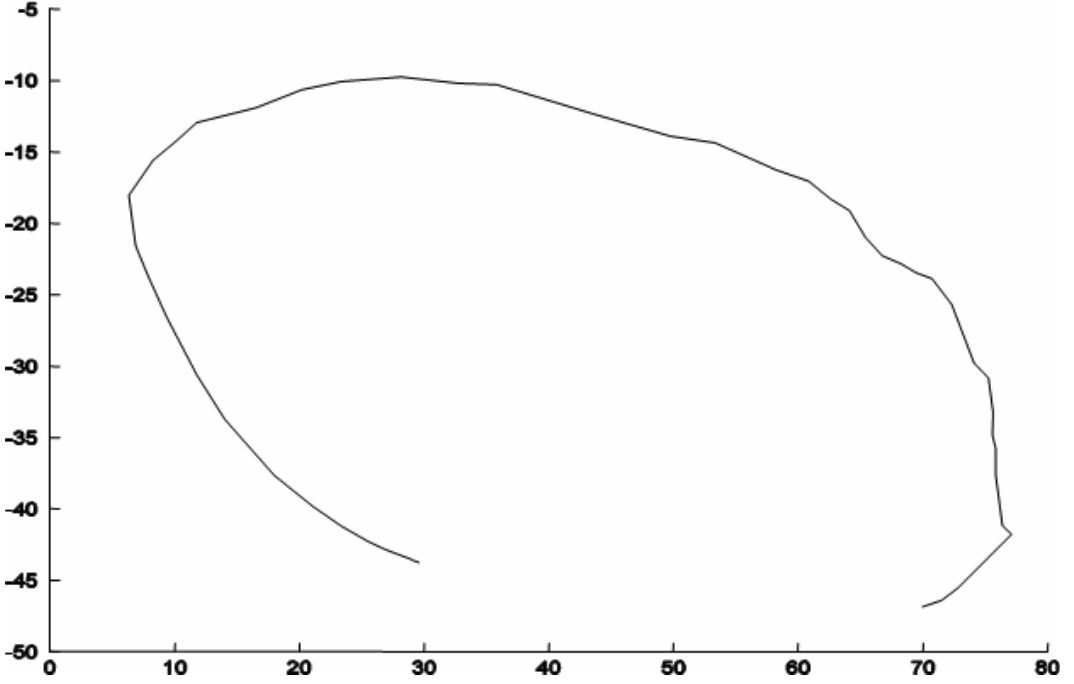
\includegraphics[width=8cm]{kearns-frontier.png}
    }
    \caption{Taken from \cite{nevmyvaka2005electronic} An illustration of the trade-off between risk and return indicated by a efficient pricing frontier.}
    \label{fig:kearns-frontier}
\end{figure}

Lastly, both techniques were combined and this resulted in an efficient pricing frontier (based on the \textit{efficient frontier} initially formulated by Harry Markowitz in 1952 \cite{markowitz1952portfolio}). 
Figure \ref{fig:kearns-frontier} shows the trade-off between the risk (x-axis) and return (y-axis).
In this example, the point of minimum risk is at $(8, 18)$ and the point of maximum returns at $(29, 9)$.
With this technique, a trader, or in our case a reinforcement learning agent, can decide upon an execution strategy by choosing how much risk and return he is willing to accept.

\section{Statistical approach}
\label{sec:related-statistical}

Substantial work in a statistical context was carried out by Chaiyakorn Yingsaeree in his dissertation \cite{yingsaeree2012algorithmic}.
A framework was proposed for the making of order placement decisions based on the trade-off between the profit gained from favorable execution prices and the risk of non-execution.
An execution probability model was developed which estimates the expected payoff (e.g. return) and its variance ($\implies$ risk) while placing orders at a certain limit level.  This is followed by the application of \textit{mean variance optimization} to balance the trade-off.
The framework was not able to beat the best static strategy in all evaluated cases, however the improvement gained when it could beat the best static strategy was very significant.
This gives us hope that, where the statistical approach has its limitations, with the reinforcement learning approach presented in this work, we may be able to understand the limitations of market data to a greater extent and avoid the shortcomings of the former strategy.
\\
\\
\textit{We are providing here an overview of the framework without specific application, as this would exceed the scope of this overview.}
\\
\\
The strategy is to buy $x$ shares in time $T$, which leaves the trader with the following options:
\begin{enumerate}
    \item Do nothing.
    \item Submit a market order at $t=0$ at price $p_{0}^M$
    \item Submit a market order at $t=T$ at price $p_{T}^M$
    \item Submit limit order at price $p^L$. If the order is not filled, either a market order follows or no action is taken (depending on the use case).
\end{enumerate}
\hfill
\\
A function $U_{E}(p)$ defines the payoff in the event of an execution at price $p$, and a function $U_{NE}(p)$ defines the cost if the order is not executed at the end of the period at market price $p$. 
Consequently, the payoff the trader will receive from submitting a limit buy order at price level $L$ is defined as,
\begin{equation}
    U(p^L) = \begin{cases}
                U_E(p), & \text{if order is executed}.\\
                U_{NE}(p_T^M), & \text{if not executed}.
             \end{cases}
\end{equation}
\hfill
\\
The expected price is compounded by a) the probability that the limit order at price $p^L$ will be executed before the end of the period and b) the distribution of the asset price at the end of the period,
\begin{equation}
    \mathbb{E}[U(p^L)] = P_E(p^L)\ U(p^L) + [1-P_E(p^L)] \int_{-\infty}^{\infty} U_{NE}(p) f_{p_M^T | p^L}(p) dp
\end{equation}
, whereas $P_E(p^L)$ is the probability that the limit order at price $p^L$ will be executed before the end of the period, and $f_{p_M^T | p^L}(.)$ is the probability density function of the asset price at the end of the period. 
\\
Similarly, the variance was defined as $V[U(p^L)]$, and this was followed by a mean variance optimization step which introduced the utility function,
\begin{equation}
    U_O(p^L) = \mathbb{E}[U(p^L)] - \lambda V[U(p^L)]
\end{equation}
, whereas $\lambda$ serves as a risk factor.
That is, when $\lambda=0$ the trader is concerned only about the profit, and when $\lambda=1$ the trader is equally concerned about profit, risk, and missed opportunities.
As a result, the trade-off between profit and risk was defined as,
\begin{equation}
    \hat{p} = \arg\max_{p^L}\ U_O(p^L)
\end{equation}


\section{Supervised Learning approach}

Fletcher et al. \cite{fletcher2010multiple} investigated order books with the aim of forecasting the movements of bid and ask prices at time $t+\Delta{t}$.
Although this was not directly applied to the optimization of order placement, the resulting predictions can certainly be used as the limit price to be set while placing an order.

SVM classification techniques with different kernels along with two Multiple Kernel Learning (MKL) techniques were used.
The authors' approach is a multi-class setup with three labels, A: $P_{t+\Delta{t}}^{Bid} > P_t^{Ask}$, B: $P_{t+\Delta{t}}^{Ask} < P_t^{Bid}$ and C: $P_{t+\Delta{t}}^{Bid} < P_t^{Ask}, P_{t+\Delta{t}}^{Ask} > P_t^{Bid}$.
The feature used is the volume at time $t$ at each of the price levels of the order book on both sides, is defined as a vector $V_t$.
A set of features was constructed that contains volumes from the current time $t$ and previous time step $t-1$.

With a time delta ($\Delta{t}$) of 100 seconds, an accuracy of 51\% was achieved.
When a shorter time delta was chosen, this resulted in significantly better performance. However, this was mostly due to the fact that the zero movement prediction was accurate.
An increased time delta resulted in significantly worse prediction accuracy.

\section{Reinforcement Learning approach}

A large-scale empirical application of reinforcement learning to optimize trade execution has been presented by Kearns et al. \cite{nevmyvaka2006reinforcement}.
Although the title of their research suggests otherwise, their work is related to order placement with a larger time horizon $H$ (2 minutes and 8 minutes), according to our definition in Section \ref{sec:execution-placement}.
Their research objective is accordingly defined as:
\begin{quote}
    to sell (or buy) V shares of a given stock within a fixed time period (or horizon) H, in a manner that maximizes the revenue received (or minimizes the capital spent).
\end{quote}
They built a reinforcement learning based on 1.5 years of millisecond time-scale limit order data from NASDAQ.
The investigation considered three stocks, AMZN, NVDA, and QCOM; each with an inventory $I$ of 5,000 shares.
The relative improvement over a submit-and-leave strategy ranged from 27.16\% to 35.50\%.
An additional improvement of 12.85\% was achieved by considering the following market variables: Spread, Immediate Cost, and Signed Volume.
\\
\\
The architecture developed is as follows.
\textit{States} are represented by a vector $x \in X$ and correspond to an observation state that has the function of making a  partially observable environment fully observable.
\textit{Actions} ($a \in A$) represent the limit price relative to the current ask price, $ask - a$. 
That is, action $a = 0$ is the ask price, $a < 0$ is a limit price deep in the book, and $a > 0$ is a limit order on the opposing side of the book.
The \textit{reward} represent the VWAP (Eq. \ref{eq:vwap}) of the executed order relative to the bid-ask mid price ($(ask + bid) / 2$).
If the order is not filled completely at the end of the time horizon H, then a market order follows.
The chosen \textit{algorithm} is a slightly adapted version of the Q-Learning algorithm that was developed by the authors, and which explores the state space inductively.
Starting from $t=T...0$ the algorithm explores the inventories $i=0...I$.
At each step, all possible actions in this state are evaluated, leading to the most rewarding strategy for $t=0$.